\documentclass[UTF8,zihao=-4]{ctexart}
\usepackage[a4paper,margin=1.9cm]{geometry}
\usepackage{hyperref}
\usepackage{array}
\usepackage{longtable}
\usepackage{verbatim}
\usepackage{xcolor}
\usepackage{graphicx}
\usepackage{tikz}
\usetikzlibrary{arrows.meta,automata,positioning}
\hypersetup{hidelinks}
\setlength{\parindent}{0pt}
\setlength{\parskip}{0.45em}
\emergencystretch=4em
\sloppy
\title{模拟卷01-2025风格题目与考试标准答案}
\author{}
\date{}
\begin{document}
\maketitle
\setcounter{tocdepth}{1}
\tableofcontents
\newpage
\section{编译原理 2025 风格模拟卷01（题目与考试标准答案）}


\subsection{卷面说明}


本卷按 Slides/Slides/handout 与三份 Recap PPT 更新，主线覆盖前端自动机与 LL、中端 IR/SSA、数据流、符号执行、后端目标代码、寄存器分配、指令调度以及过程间/指针分析。总分 100 分。


\section{A 卷题目}


\subsection{一、词法分析（15 分）}


正则表达式：


\begin{quote}
\footnotesize
\begin{verbatim}
(epsilon|y)* x y*
\end{verbatim}
\end{quote}


\begin{enumerate}
\item 使用 Thompson 构造法构造等价 NFA。
\item 使用子集构造法构造 DFA，写明 DFA 状态含义。
\item 最小化 DFA。
\end{enumerate}


\subsection{二、LL 语法分析（15 分）}


文法：


\begin{quote}
\footnotesize
\begin{verbatim}
A -> B C
B -> B P | r
C -> t | u
\end{verbatim}
\end{quote}


\begin{enumerate}
\item 消除左递归。
\item 写 FIRST 和 FOLLOW。
\item 写预测分析表。
\item 判断消除左递归后的文法是否为 LL(1)。
\end{enumerate}


\subsection{三、指令调度（15 分）}


给定指令：


\begin{quote}
\footnotesize
\begin{verbatim}
I1: R1 = R2 + R3
I2: R4 = R1 + R5
I3: R2 = R6 + R7
I4: R1 = R8 + R9
I5: R10 = R4 + R1
\end{verbatim}
\end{quote}


\begin{enumerate}
\item 写出指令调度的目的。
\item 写出 RAW、WAR、WAW 的定义。
\item 构建依赖图，WAR/WAW 用虚线表示。
\item 在允许寄存器重命名的条件下给出一个合法重排序列。
\end{enumerate}


\subsection{四、支配问题（15 分）}


CFG：菱形分支


\begin{quote}
\footnotesize
\begin{verbatim}
Entry->B1
B1->B2
B1->B3
B2->B4
B3->B4
B4->Exit
\end{verbatim}
\end{quote}


\begin{enumerate}
\item 写出 Dom、PostDom、Dom Frontier 的定义。
\item 计算每个节点的 Dom 集和 idom。
\item 写出支配边界。
\item 说明 SSA 中 phi 函数应放在什么位置。
\end{enumerate}


\subsection{五、符号执行与 SAT（20 分）}


公式：


\begin{quote}
\footnotesize
\begin{verbatim}
F = ((a1 and b1) or c1)
\end{verbatim}
\end{quote}


\begin{enumerate}
\item 写出 Path-sensitive、Flow-sensitive、Context-sensitive 的定义。
\item 写出 CNF 的定义。
\item 使用 Tseitin 算法把 F 转成 CNF。
\item 证明 2025 卷中的两组公式同时可满足。
\end{enumerate}


\subsection{六、Andersen 指针分析（20 分）}


程序：


\begin{quote}
\footnotesize
\begin{verbatim}
p = &a
q = &b
*p = q
r = &c
s = p
t = *p
*s = r
\end{verbatim}
\end{quote}


\begin{enumerate}
\item 对每条语句写 Andersen 约束。
\item 根据约束构建闭包。
\item 写出最终 points-to 集合。
\end{enumerate}


\subsection{七、PPT 新增重点：数据流分析（10 分）}


CFG 与可达定值信息：

\begin{quote}
\footnotesize
\begin{verbatim}
Entry->B1
B1->B2
B2->B3
B2->B4
B3->B4

B1: gen={d1}, kill={}
B2: gen={d2}, kill={d1}
B3: gen={d3}, kill={}
B4: gen={d4}, kill={d2}
\end{verbatim}
\end{quote}


\begin{enumerate}
\item 写出 Reaching Definitions 的方向、meet 和 transfer 方程。
\item 计算各基本块的 IN/OUT。
\item 说明 worklist 算法什么时候停止。

\end{enumerate}

\section{B 按考试标准重写答案}


\subsection{一、词法分析答案}


\begin{quote}
\footnotesize
\begin{verbatim}
正则表达式：(epsilon|y)* x y*

Thompson NFA：起点 q0，终点 q11。图中 q11 画双圈，下面转移表与图一致。
\end{verbatim}

\begin{center}
\resizebox{\linewidth}{!}{%
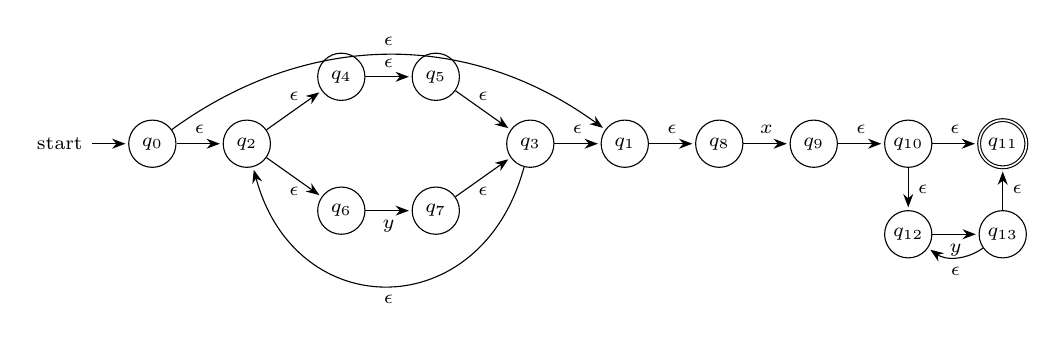
\begin{tikzpicture}[
  >=Stealth,
  shorten >=1pt,
  auto,
  every state/.style={minimum size=6mm, inner sep=0pt},
  every edge/.style={draw, ->},
  font=\scriptsize
]
\node[state, initial] (q0) at (0,0) {$q_0$};
\node[state] (q2) at (1.2,0) {$q_2$};
\node[state] (q4) at (2.4,0.85) {$q_4$};
\node[state] (q5) at (3.6,0.85) {$q_5$};
\node[state] (q3) at (4.8,0) {$q_3$};
\node[state] (q6) at (2.4,-0.85) {$q_6$};
\node[state] (q7) at (3.6,-0.85) {$q_7$};
\node[state] (q1) at (6.0,0) {$q_1$};
\node[state] (q8) at (7.2,0) {$q_8$};
\node[state] (q9) at (8.4,0) {$q_9$};
\node[state] (q10) at (9.6,0) {$q_{10}$};
\node[state, accepting] (q11) at (10.8,0) {$q_{11}$};
\node[state] (q12) at (9.6,-1.15) {$q_{12}$};
\node[state] (q13) at (10.8,-1.15) {$q_{13}$};
\path[->]
  (q0) edge node[above] {$\epsilon$} (q2)
  (q0) edge[bend left=36] node[above] {$\epsilon$} (q1)
  (q2) edge node[above] {$\epsilon$} (q4)
  (q4) edge node[above] {$\epsilon$} (q5)
  (q5) edge node[above] {$\epsilon$} (q3)
  (q2) edge node[below] {$\epsilon$} (q6)
  (q6) edge node[below] {$y$} (q7)
  (q7) edge node[below] {$\epsilon$} (q3)
  (q3) edge[out=-105,in=-75,looseness=1.55] node[below] {$\epsilon$} (q2)
  (q3) edge node[above] {$\epsilon$} (q1)
  (q1) edge node[above] {$\epsilon$} (q8)
  (q8) edge node[above] {$x$} (q9)
  (q9) edge node[above] {$\epsilon$} (q10)
  (q10) edge node[right] {$\epsilon$} (q12)
  (q10) edge node[above] {$\epsilon$} (q11)
  (q12) edge node[below] {$y$} (q13)
  (q13) edge[bend left=35] node[below] {$\epsilon$} (q12)
  (q13) edge node[right] {$\epsilon$} (q11);
\end{tikzpicture}%
}
\end{center}

子集构造 DFA 和最小 DFA 图如下。图后的状态集合与分组仍保留，便于核对。

\begin{center}
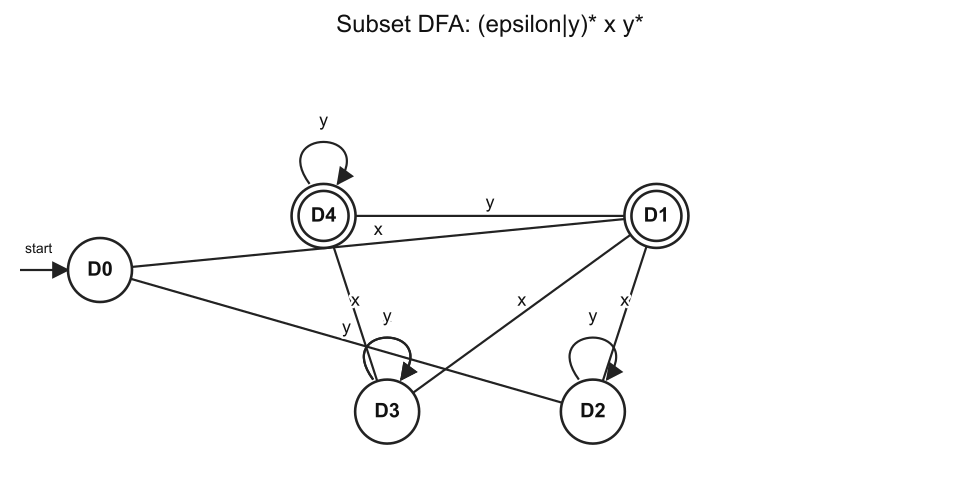
\includegraphics[width=0.88\linewidth]{figures/mock01-dfa.png}

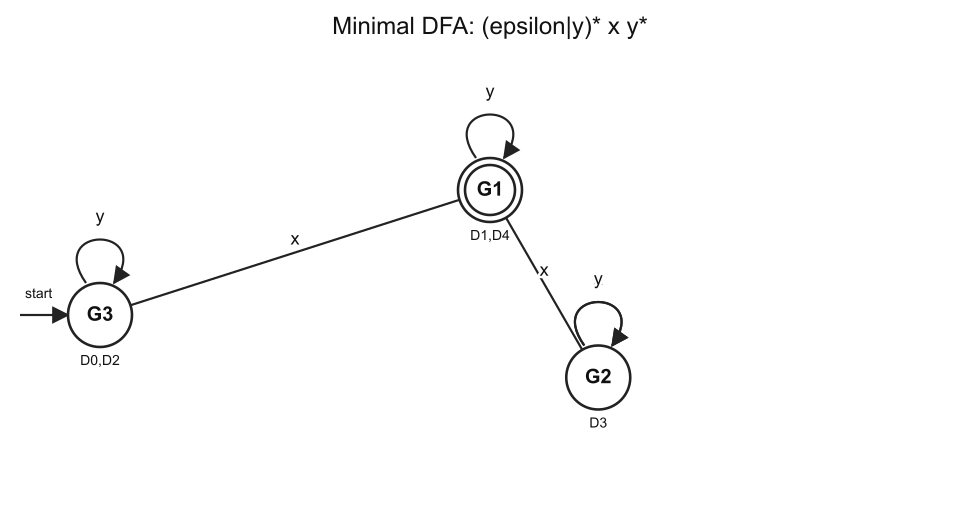
\includegraphics[width=0.88\linewidth]{figures/mock01-min-dfa.png}
\end{center}

\begin{verbatim}
Thompson NFA 转移表：
q4 --epsilon--> q5
q6 --y--> q7
q2 --epsilon--> q4
q2 --epsilon--> q6
q5 --epsilon--> q3
q7 --epsilon--> q3
q0 --epsilon--> q2
q0 --epsilon--> q1
q3 --epsilon--> q2
q3 --epsilon--> q1
q8 --x--> q9
q1 --epsilon--> q8
q12 --y--> q13
q10 --epsilon--> q12
q10 --epsilon--> q11
q13 --epsilon--> q12
q13 --epsilon--> q11
q9 --epsilon--> q10

子集构造 DFA：
D0:
  NFA集合 = {q0,q1,q2,q3,q4,q5,q6,q8}
  on x -> D1
  on y -> D2
  终态 = 否
D1:
  NFA集合 = {q9,q10,q11,q12}
  on x -> D3
  on y -> D4
  终态 = 是
D2:
  NFA集合 = {q1,q2,q3,q4,q5,q6,q7,q8}
  on x -> D1
  on y -> D2
  终态 = 否
D3:
  NFA集合 = EMPTY
  on x -> D3
  on y -> D3
  终态 = 否
D4:
  NFA集合 = {q11,q12,q13}
  on x -> D3
  on y -> D4
  终态 = 是

最小化：
初分组：
  终态组 = {D1,D4}
  非终态组 = {D0,D2,D3}
最终分组：
  G1 = {D1,D4}
  G2 = {D3}
  G3 = {D0,D2}
每个最终分组对应一个最小 DFA 状态。
\end{verbatim}
\end{quote}

最小化推理过程：

\begin{center}
\footnotesize
\begin{tabular}{llll}
\hline
状态集合 & 输入 x 后 & 输入 y 后 & 结论 \\
\hline
\{D1,D4\} & 都到 \{D3\} & 都到 \{D1,D4\} & D1、D4 可合并 \\
\{D0,D2\} & 都到 \{D1,D4\} & 都到 \{D0,D2\} & D0、D2 可合并 \\
\{D3\} & 到自身 & 到自身 & 与 D0、D2 在 x 上不同，单独成组 \\
\hline
\end{tabular}
\end{center}

因此最小 DFA 有 3 个状态：G3=\{D0,D2\} 为初态，G1=\{D1,D4\} 为终态，G2=\{D3\} 为死状态。



\subsection{二、LL 语法分析答案}


\begin{quote}
\footnotesize
\begin{verbatim}
原文法：
A -> B C
B -> B P | r
C -> t | u

消除左递归：
A  -> B C
B  -> r B'
B' -> P B' | epsilon
C  -> t | u

FIRST：
FIRST(A)={ r }
FIRST(B)={ r }
FIRST(B')={ P, epsilon }
FIRST(C)={ t, u }

FOLLOW：
FOLLOW(A)={ $ }
FOLLOW(B)={ t, u }
FOLLOW(B')={ t, u }
FOLLOW(C)={ $ }

预测表：
M[A,r] = A -> B C
M[B,r] = B -> r B'
M[B',P] = B' -> P B'
M[B',t] = B' -> epsilon
M[B',u] = B' -> epsilon
M[C,t] = C -> t
M[C,u] = C -> u

结论：表中无多重入口，消除左递归后的文法是 LL(1)。
\end{verbatim}
\end{quote}

预测分析表（表格形式）：

\begin{center}
\footnotesize
\begin{tabular}{lll}
\hline
非终结符 & 输入符号 & 产生式 \\
\hline
A & r & A -> B C \\
B & r & B -> r B' \\
B' & P & B' -> P B' \\
B' & t & B' -> epsilon \\
B' & u & B' -> epsilon \\
C & t & C -> t \\
C & u & C -> u \\
\hline
\end{tabular}
\end{center}

填表推导过程：

\begin{quote}
\footnotesize
\begin{verbatim}
B -> B P | r 是直接左递归。
按 A -> A alpha | beta 改写为：
A  -> beta A'
A' -> alpha A' | epsilon

这里 alpha=P，beta=r，
所以 B -> r B'，B' -> P B' | epsilon。

FIRST(B)={r}
FIRST(B')={P, epsilon}
FIRST(C)={t,u}
FIRST(A)=FIRST(B C)=FIRST(B)={r}

FOLLOW(A)={$}
由 A -> B C 得 FIRST(C) 加入 FOLLOW(B)，所以 FOLLOW(B)={t,u}
由 B -> r B' 得 FOLLOW(B) 加入 FOLLOW(B')，所以 FOLLOW(B')={t,u}
由 A -> B C 得 FOLLOW(A) 加入 FOLLOW(C)，所以 FOLLOW(C)={$}
\end{verbatim}
\end{quote}

完整预测分析表，空白项为 error：

\begin{center}
\footnotesize
\begin{tabular}{llllll}
\hline
非终结符 & r & P & t & u & \$ \\
\hline
A & A -> B C & error & error & error & error \\
B & B -> r B' & error & error & error & error \\
B' & error & B' -> P B' & B' -> epsilon & B' -> epsilon & error \\
C & error & error & C -> t & C -> u & error \\
\hline
\end{tabular}
\end{center}

每个表项最多只有一条产生式，因此消除左递归后的文法是 LL(1)。



\subsection{三、指令调度答案}


定义：


\begin{quote}
\footnotesize
\begin{verbatim}
指令调度在不改变程序语义的前提下重排指令，减少流水线停顿，提高并行执行效率。
RAW：先写后读，必须保持顺序。
WAR：先读后写，写者不能提前。
WAW：先写后写，顺序影响最终值。
\end{verbatim}
\end{quote}


\begin{quote}
\footnotesize
\begin{verbatim}
指令：
I1: R1 = R2 + R3
I2: R4 = R1 + R5
I3: R2 = R6 + R7
I4: R1 = R8 + R9
I5: R10 = R4 + R1

依赖：
I1 -> I2 RAW on R1
I1 -> I3 WAR on R2
I1 -> I4 WAW on R1
I2 -> I4 WAR on R1
I2 -> I5 RAW on R4
I4 -> I5 RAW on R1

寄存器重命名：
I3: R2_new = R6 + R7
I4: R1_new = R8 + R9
I5 使用 R1_new

重命名后保留 RAW，WAR/WAW 被消除。一个合法调度序列：
I1, I3, I4, I2, I5
\end{verbatim}
\end{quote}

读写集合：

\begin{center}
\footnotesize
\begin{tabular}{lll}
\hline
指令 & 读寄存器 & 写寄存器 \\
\hline
I1 & R2, R3 & R1 \\
I2 & R1, R5 & R4 \\
I3 & R6, R7 & R2 \\
I4 & R8, R9 & R1 \\
I5 & R4, R1 & R10 \\
\hline
\end{tabular}
\end{center}

逐对检查依赖：

\begin{center}
\footnotesize
\begin{tabular}{llll}
\hline
依赖边 & 类型 & 寄存器 & 判断逻辑 \\
\hline
I1 -> I2 & RAW & R1 & I1 写 R1，I2 读 R1 \\
I1 -> I3 & WAR & R2 & I1 读 R2，I3 后写 R2 \\
I1 -> I4 & WAW & R1 & I1 写 R1，I4 后写 R1 \\
I2 -> I4 & WAR & R1 & I2 读 R1，I4 后写 R1 \\
I2 -> I5 & RAW & R4 & I2 写 R4，I5 读 R4 \\
I4 -> I5 & RAW & R1 & I4 写 R1，I5 读 R1 \\
\hline
\end{tabular}
\end{center}

依赖图如下。实线是 RAW，虚线是 WAR/WAW：

\begin{center}
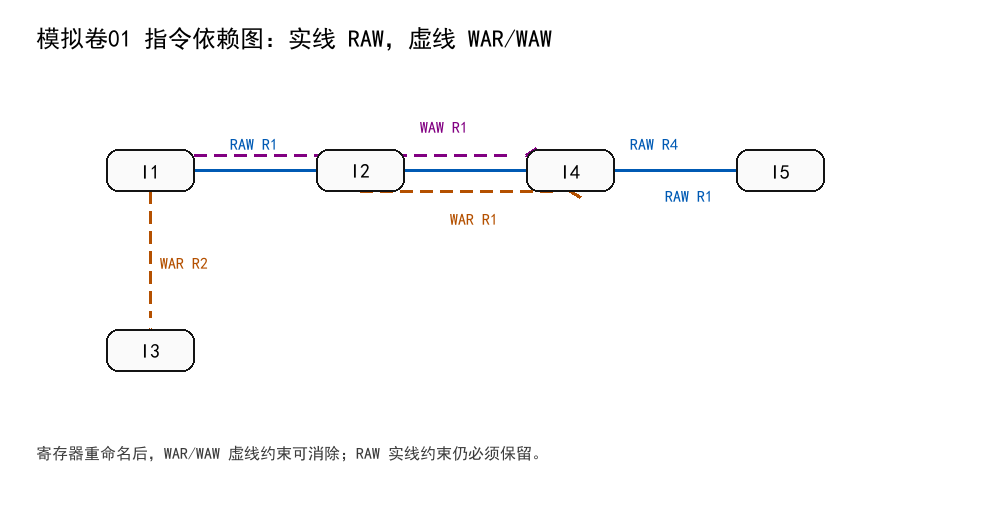
\includegraphics[width=0.9\linewidth]{figures/mock01-instruction-dependencies.png}
\end{center}

寄存器重命名后，I3 写 R2\_new，I4 写 R1\_new，I5 使用 R1\_new。此时 WAR/WAW 虚线约束被消除，仍需满足 I1 -> I2、I2 -> I5、I4 -> I5。序列 I1, I3, I4, I2, I5 满足这些 RAW 约束，所以是合法调度。



\subsection{四、支配问题答案}


定义：


\begin{quote}
\footnotesize
\begin{verbatim}
Dom(n)：入口到 n 的每条路径都经过的节点集合。
PostDom(n)：n 到出口的每条路径都经过的节点集合。
Dom Frontier(n)：n 支配某个前驱，但不严格支配该节点的位置。
\end{verbatim}
\end{quote}


\begin{quote}
\footnotesize
\begin{verbatim}
CFG 边：
Entry->B1
B1->B2
B1->B3
B2->B4
B3->B4
B4->Exit

Dom 集：
Dom(Entry)={Entry}
Dom(B1)={Entry,B1}
Dom(B2)={Entry,B1,B2}
Dom(B3)={Entry,B1,B3}
Dom(B4)={Entry,B1,B4}
Dom(Exit)={Entry,B1,B4,Exit}

直接支配者：
idom(B1)=Entry
idom(B2)=B1
idom(B3)=B1
idom(B4)=B1
idom(Exit)=B4

支配边界：
DF(B2)={B4}
DF(B3)={B4}
其余节点 DF 为空集

SSA phi 放置：若变量在多个基本块中被定义，则在这些定义块的迭代支配边界处插入该变量的 phi。直观上，phi 放在多条控制流汇合且不同定义可能到达的位置。
\end{verbatim}
\end{quote}

CFG 图如下：

\begin{center}
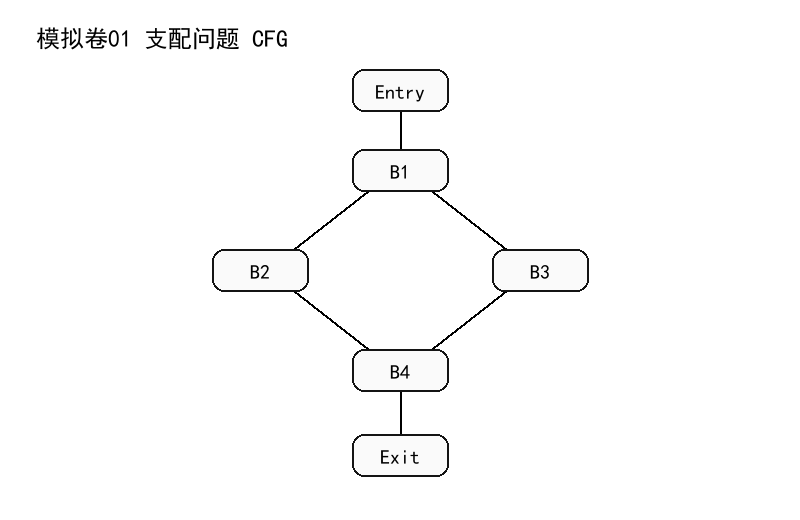
\includegraphics[width=0.72\linewidth]{figures/mock01-diamond-cfg.png}
\end{center}

Dom 集按方程 Dom(n)=\{n\} union intersection(Dom(p)) 逐点计算：

\begin{center}
\footnotesize
\begin{tabular}{llll}
\hline
节点 & 前驱 & 计算过程 & Dom 集 \\
\hline
Entry & 无 & 入口固定 & \{Entry\} \\
B1 & Entry & \{B1\} union Dom(Entry) & \{Entry,B1\} \\
B2 & B1 & \{B2\} union Dom(B1) & \{Entry,B1,B2\} \\
B3 & B1 & \{B3\} union Dom(B1) & \{Entry,B1,B3\} \\
B4 & B2,B3 & \{B4\} union (Dom(B2) intersection Dom(B3)) & \{Entry,B1,B4\} \\
Exit & B4 & \{Exit\} union Dom(B4) & \{Entry,B1,B4,Exit\} \\
\hline
\end{tabular}
\end{center}

支配边界判断：

\begin{center}
\footnotesize
\begin{tabular}{lll}
\hline
节点 & 判断 & 支配边界 \\
\hline
B2 & B2 支配 B4 的前驱 B2，但不严格支配 B4 & \{B4\} \\
B3 & B3 支配 B4 的前驱 B3，但不严格支配 B4 & \{B4\} \\
Entry, B1, B4, Exit & 不满足支配边界条件 & \{\} \\
\hline
\end{tabular}
\end{center}

因此若某变量在 B2、B3 两个分支中都有定义，则该变量的 phi 应插入 B4。



\subsection{五、符号执行与 SAT 答案}


\begin{quote}
\footnotesize
\begin{verbatim}
公式：F = ((a1 and b1) or c1)
引入：x11 <-> (a1 and b1)，x12 <-> (x11 or c1)，根变量 x12 为真。

CNF：
(not x11 or a1)
(not x11 or b1)
(x11 or not a1 or not b1)
(x12 or not x11)
(x12 or not c1)
(not x12 or x11 or c1)
(x12)

敏感性定义：
Path-sensitive 区分不同路径。
Flow-sensitive 区分程序点和语句顺序。
Context-sensitive 区分函数调用上下文。

同时可满足证明套用：
F1=(a0 or ... or an or c) and (b0 or ... or bm or not c)，F2=(a0 or ... or an or b0 or ... or bm)。
F1 为真时，c=false 推出某个 ai=true，c=true 推出某个 bj=true，所以 F2 为真。
F2 为真时，若某个 ai=true 令 c=false；若某个 bj=true 令 c=true，所以 F1 为真。
\end{verbatim}
\end{quote}

Tseitin 转换的推导表：

\begin{center}
\footnotesize
\begin{tabular}{lll}
\hline
子公式 & 新变量 & 产生的 CNF 子句 \\
\hline
a1 and b1 & x11 & (not x11 or a1); (not x11 or b1); (x11 or not a1 or not b1) \\
x11 or c1 & x12 & (x12 or not x11); (x12 or not c1); (not x12 or x11 or c1) \\
根公式为真 & x12 & (x12) \\
\hline
\end{tabular}
\end{center}

同时可满足证明按两个方向写：F1 为真时，若 c=false，则第一项必须由某个 ai=true 保证；若 c=true，则第二项必须由某个 bj=true 保证，因此 F2 为真。反过来，F2 为真时，若有某个 ai=true，取 c=false；若有某个 bj=true，取 c=true，均可使 F1 为真。



\subsection{六、Andersen 指针分析答案}


\begin{quote}
\footnotesize
\begin{verbatim}
程序：
p = &a
q = &b
*p = q
r = &c
s = p
t = *p
*s = r

约束：
a in pts(p)
b in pts(q)
for v in pts(p), pts(q) subset pts(v)
c in pts(r)
pts(p) subset pts(s)
for v in pts(p), pts(v) subset pts(t)
for v in pts(s), pts(r) subset pts(v)

闭包：
pts(p)={a}
pts(q)={b}
pts(r)={c}
pts(s)={a}
由 *p=q 得 pts(a) 包含 {b}
由 *s=r 得 pts(a) 包含 {c}
由 t=*p 得 pts(t) 包含 pts(a)，最终 pts(t)={b,c}
最终 pts(a)={b,c}
\end{verbatim}
\end{quote}

逐条语句生成约束：

\begin{center}
\footnotesize
\begin{tabular}{lll}
\hline
语句 & Andersen 约束 & 含义 \\
\hline
p = \&a & a in pts(p) & p 指向 a \\
q = \&b & b in pts(q) & q 指向 b \\
*p = q & 对 v in pts(p)，pts(q) subset pts(v) & q 的指向流入 p 所指对象 \\
r = \&c & c in pts(r) & r 指向 c \\
s = p & pts(p) subset pts(s) & p 的指向流入 s \\
t = *p & 对 v in pts(p)，pts(v) subset pts(t) & p 所指对象内容流入 t \\
*s = r & 对 v in pts(s)，pts(r) subset pts(v) & r 的指向流入 s 所指对象 \\
\hline
\end{tabular}
\end{center}

闭包计算过程：

\begin{center}
\footnotesize
\begin{tabular}{lll}
\hline
轮次 & 新增事实 & 原因 \\
\hline
0 & pts(p)=\{a\}, pts(q)=\{b\}, pts(r)=\{c\} & 取地址语句 \\
1 & pts(s)=\{a\} & s = p \\
2 & pts(a) 加入 b & *p = q，且 pts(p)=\{a\} \\
3 & pts(a) 加入 c & *s = r，且 pts(s)=\{a\} \\
4 & pts(t)=\{b,c\} & t = *p，且 pts(a)=\{b,c\} \\
\hline
\end{tabular}
\end{center}

最终 points-to 集合为：pts(p)=\{a\}，pts(q)=\{b\}，pts(r)=\{c\}，pts(s)=\{a\}，pts(t)=\{b,c\}，pts(a)=\{b,c\}。



\subsection{七、PPT 新增重点答案}


\begin{quote}
\footnotesize
\begin{verbatim}
Reaching Definitions：
方向：前向。
meet：并集 union。
transfer：OUT[B] = gen[B] union (IN[B] - kill[B])
入口：IN[B1] = {}

IN[B1]  = {}
OUT[B1] = {d1}

IN[B2]  = OUT[B1] = {d1}
OUT[B2] = {d2}

IN[B3]  = OUT[B2] = {d2}
OUT[B3] = {d2,d3}

IN[B4]  = OUT[B2] union OUT[B3] = {d2,d3}
OUT[B4] = {d3,d4}

worklist 停止条件：所有基本块重新计算后 IN/OUT 都不再变化。
\end{verbatim}
\end{quote}

数据流图如下：

\begin{center}
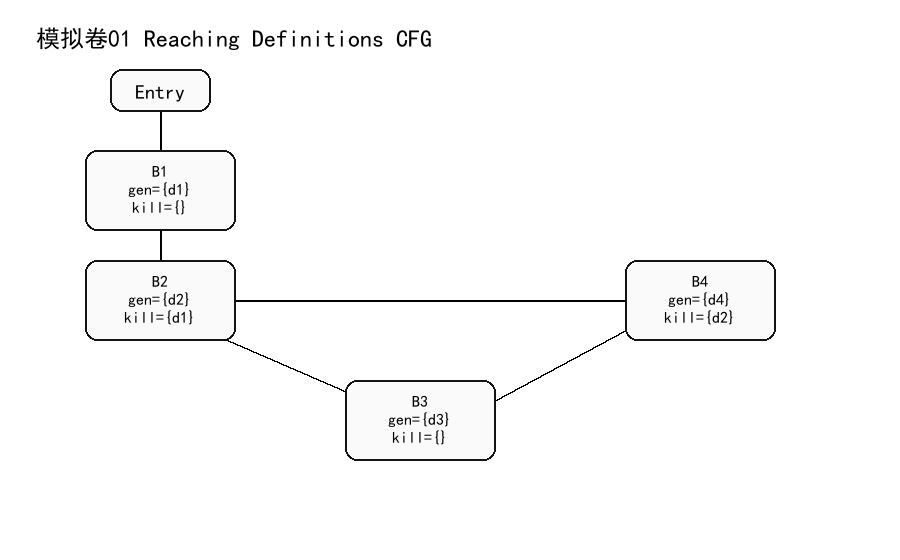
\includegraphics[width=0.88\linewidth]{figures/mock01-dataflow-cfg.png}
\end{center}

按方程 IN[B]=union OUT[P]，OUT[B]=gen[B] union (IN[B]-kill[B]) 代入：

\begin{center}
\footnotesize
\begin{tabular}{lll}
\hline
基本块 & IN & OUT \\
\hline
B1 & \{\} & \{d1\} \\
B2 & \{d1\} & \{d2\} \\
B3 & \{d2\} & \{d2,d3\} \\
B4 & \{d2,d3\} & \{d3,d4\} \\
\hline
\end{tabular}
\end{center}

worklist 算法停止条件不是访问完一遍，而是某轮重新计算后所有基本块的 IN/OUT 都不再变化。
\end{document}
